\documentclass[a4paper]{article}
\usepackage[backend=bibtex]{biblatex}
\usepackage[utf8]{inputenc}
\usepackage{soul,xcolor}
\usepackage{rotating}
\usepackage{ulem}
\usepackage{lineno, blindtext}
\usepackage{etoolbox}
\usepackage{nopageno}
\usepackage{parskip}
\usepackage{transparent}
\usepackage{xcolor}
\usepackage[paperwidth=5.5in, paperheight=10in,  top=0.1in, bottom=0.1in, left=0.6in, right=0.4in]{geometry}
\usepackage[absolute]{textpos}
\usepackage{tikz}
\usepackage{circledsteps}
\usepackage{stackengine}
\usepackage{stix}
\usetikzlibrary{arrows.meta,decorations.pathreplacing,calligraphy}

\newcommand{\ulfelttip}[1]{%
    \tikz[baseline=(to_underline.base)]{
        \node[inner sep=0pt,outer sep=0pt] (to_underline) {#1};
        \color{red}
        \draw[line width=0.05in, opacity=0.6] ([xshift=1pt,yshift=-2pt]to_underline.south west) -- ([xshift=-1pt,yshift=-2pt]to_underline.south east);
    }%
}%

\newcommand{\multilinebrace}{
	
\begin{tikzpicture}[remember picture,overlay]
		\draw [pen colour ={blue},
		decorate, 
		decoration = {calligraphic brace}
		] (-0.2,-1.3) -- (-0.2,0.3);
	\end{tikzpicture}
}

\newcommand{\multilineclamp}{
	\begin{tikzpicture}[remember picture,overlay,line width=0.05in,opacity=0.6]
                \draw (0.5, 0.4) --  (-0.7,0.4) -- (-0.7, -2.2) -- (-0.9, -2.2);
                \draw (-0.7, -2.75) -- (-0.7, -6.5); 
                \draw[<-] (-0.7,-7.7) -- (-0.7, -11) -- (0.7, -11);
        \end{tikzpicture}
}

\newcommand{\bigcross}{
	
\begin{tikzpicture}[remember picture,overlay]
		\draw (-0.8,1.3) -- (0.8,-1.3);
		\draw (0.8, 1.5) -- (-0.8,-1.3);
	\end{tikzpicture}
}

\newcommand{\mediumcrossright}{
	\begin{tikzpicture}[remember picture,overlay]
		\draw (0.5,0.2) -- (0.8,-0.1);
		\draw (0.8, 0.2) -- (0.5,-0.1);
	\end{tikzpicture}
}

\newcommand{\mediumcrossabove}{
	
\begin{tikzpicture}[remember picture,overlay]
		\draw (-0.15,0.5) -- (0.15,0.2);
		\draw (0.15, 0.5) -- (-0.15,0.2);
	\end{tikzpicture}
}

\newcommand{\mediumcrossaboveright}{
	\begin{tikzpicture}[remember picture,overlay]
		\draw (0.5,0.5) -- (0.8,0.2);
		\draw (0.8, 0.5) -- (0.5,0.2);
	\end{tikzpicture}
}

\newcommand{\smalltickright}{
	\begin{tikzpicture}[remember picture,overlay]
		\draw (0.3,0) -- (0.4,-0.2);
		\draw (0.4,-0.2) -- (1.1,0.5);
	\end{tikzpicture}
}

\newcommand{\lineofsmallticks}{
	\begin{tikzpicture}[remember picture,overlay]
		\draw (0.3,0) -- (0.4,-0.1);
		\draw (0.4,-0.1) -- (0.8,0.4);
                \draw (1.2,0) -- (1.3,-0.1);
		\draw (1.3,-0.1) -- (1.7,0.4);
                \draw (2.4,0) -- (2.5,-0.1);
		\draw (2.5,-0.1) -- (2.9,0.4);
                \draw (3.3,0) -- (3.4,-0.1);
		\draw (3.4,-0.1) -- (3.8,0.4);
	\end{tikzpicture}
}

\newcommand{\mediumtickright}{
	\begin{tikzpicture}[remember picture,overlay]
		\draw (0.3,0) -- (0.4,-0.2);
		\draw (0.4,-0.2) -- (1.5,0.9);
	\end{tikzpicture}
}

\newcommand{\mediumtickrightunder}{
	\begin{tikzpicture}[remember picture,overlay]
		\draw (0.4,-0.3) -- (0.5,-0.5);
		\draw (0.5,-0.5) -- (1.5,0.4);
	\end{tikzpicture}
}

\newcommand{\bigtickdeep}{
	
\begin{tikzpicture}[remember picture,overlay]
		\draw (-0.2,0.1) -- (0.2,-0.6);
		\draw (0.2,-0.6) -- (1.1,1.2);
	\end{tikzpicture}
}

\newcommand{\bigtickshallow}{
	
\begin{tikzpicture}[remember picture,overlay]
		\draw (-0.1,0) -- (0.1,-0.2);
		\draw (0.1,-0.2) -- (3,2.2);
	\end{tikzpicture}
}

\newcommand{\gianttick}{
	
\begin{tikzpicture}[remember picture,overlay]
		\draw (0.1,0) -- (0.3,-0.2);
		\draw (0.3,-0.2) -- (5,5);
	\end{tikzpicture}
}

\newcommand{\liketovenusarrow}{
        \begin{tikzpicture}[remember picture,overlay]
                \draw (0.5,0.25) -- (-0.1, 0.25) -- (-0.1,-0.15) -- (0.5, -0.15);
                \draw[->] (-0.1,0) .. controls (-4,-1.5) .. (-3.5,-4);
        \end{tikzpicture}
}

\newcommand{\cymbelineline}{
        \begin{tikzpicture}[remember picture,overlay]
                \draw (-0.1,-0.05) -- (-0.55, -0.2);
        \end{tikzpicture}
}

\setlength{\parindent}{0pt}
\preto{\draft}{\resetlinenumber}
\renewcommand{\linenumberfont}{\normalfont\bfseries\small\color{red}}
\setstcolor{red}
\begin{document}
% \colorbox{gray}{
\begin{minipage}{0.1\textwidth}
\Circled{\color{blue}{13}} 
\end{minipage}
\begin{minipage}{0.2\textwidth}
\color{blue}
\small
\null list \#11\par
b. July 22/75
\end{minipage}
% }
% \colorbox{orange}{
\begin{minipage}{0.7\textwidth}
\color{blue}
\begin{flushright}
\Circled{p.19}\par
\end{flushright}
\hspace{1cm}
Gray
$\rightarrow$
\color{red}\Circled{\color{blue}{Venus's Looking-glass}}\par
\end{minipage}

\color{blue}
\begin{minipage}[t]{0.3\textwidth}
%lh column
\setulcolor{red}
Gray: \ulfelttip{corolla}\par
of $\color{red}\smalltickright$\ulfelttip{perfect} $\color{red}\smalltickright$\ulfelttip{flowers}\par
\ulfelttip{rotate} \ulfelttip{5-lobed};\par
fertilized\par
$\color{red}\smalltickright$\ulfelttip{unopening} \&\par
greatly reduced\par
flowers $\color{red}\smalltickright$\ulfelttip{in} \ulfelttip{lower}\par
$\color{red}\mediumtickright$\ulfelttip{axils}; capsule\par
prismatic, cylindric\par
to awl shaped 3-\par
locular, opening\par
by 3 sma$\color{red}\bigcross$ll lateral\par
valves above the\par
middle; \ulfelttip{axillary}\par
\ulfelttip{blue} + \ulfelttip{purplish}\par %"or" in Gray; might be misreading here
flowers earlier\par
Euro$\color{red}\mediumtickright$pean name\par
\ul{Specul\`aria Speculum-}\par
$\color{red}\mediumtickright$\ul{Veneris}, mirror of V.\par
var \ulfelttip{Spec}\ul{ularia} $\color{red}\mediumcrossright$\ul{perfoliata}:\par
\ulfelttip{leaves} $\color{red}\smalltickright$\ulfelttip{clasping}, about as\par
broad as long, expanded\par
corollas usually borne\par
at several upper nodes\par
capsule$\color{red}\bigtickdeep$ pores 
\setulcolor{blue}\ul{sub}-\par
median\par
\vspace{0.2cm}
\small
\sout{Taylor}\par
\normalsize
%LZ takes part on perfoliata from distinction guide rather than longer entry on perfoliata. Use of Gray to do with process of finding out rather than/as much as source of knowledge
\end{minipage}
\hspace{1cm}
%main rh column
\begin{minipage}[t]{10cm}
\vspace{3cm}
\ul{Field Flowers}
\setulcolor{red}
illust.p9 \ul{Specularia}\par
\savestack{\specularianote}{\Longstack[r]{ {$\color{red}\mediumcrossright$\ul{perfoliata} $\color{red}\mediumtickrightunder$(Belleflower}}}%
\hspace{3cm}\Longunderstack[r]{{\specularianote}  {f.)} }\par 
\setul{}{2pt}
has \ulfelttip{two} \ulfelttip{kinds}$\color{red}\bigtickshallow$ \ulfelttip{of flowers} .. \ulfelttip{earliest}\par
borne \ulfelttip{on} \ulfelttip{lower part} \ulfelttip{of stems} .. insignificant\par
in appearance .. set \ulfelttip{seeds} \ulfelttip{without} recvg\par
\ulfelttip{pollen from} \ulfelttip{other} \ulfelttip{flowers} .. the \ulfelttip{later ones}\par
\ulfelttip{higher up} .. showy .. \ulfelttip{visited} by \ulfelttip{insects}\par
\ulfelttip{which} carry \ulfelttip{pollen} \ulfelttip{from} \ulfelttip{one} to \ulfelttip{the other} \& \ulfelttip{bring}\par
\ulfelttip{about} \ulfelttip{cross}-\ulfelttip{fertilization}. Season:\par
\ulfelttip{May}-\ulfelttip{Sept}. Flowers: \ulfelttip{solitary} or \ulfelttip{2 or} 3\par
\ulfelttip{together} .. 5 (\ulfelttip{rarely} 4) \ulfelttip{reddish-violet} \ulfelttip{petals}\par
annual 6 in to 2ft \ulfelttip{tall stems} \ulfelttip{rather}\par
\ulfelttip{weak} $\color{red}\gianttick$\ulfelttip{Leaves shell-shaped} \ulfelttip{stem}\ulfelttip{-clasping}\par
1" or less D.\par 
\end{minipage}

% absolute positioned boxes

%lh column

\begin{textblock*}{3cm}(2.5cm,14cm)%
	\begin{minipage}{3cm} 
        \color{red}
        \transparent{0.6}
        \textbf{Bell-looking-glass}\par
        \textbf{(one word}\par
        $\color{blue}\mediumtickright$\textbf{2 hyphens)}\par
	\end{minipage}%
\end{textblock*}%

\begin{textblock*}{3cm}(5cm,14.5cm)%
	\begin{minipage}{3cm} 
        \color{red}
        \transparent{0.6}
        % ideally circle would be same thickness/opacity
        % but doesn't look trivial from a quick look at
        % package docs
        \huge \Circled{$\ast$}\par
	\end{minipage}%
\end{textblock*}%

\begin{textblock*}{3cm}(4cm,18.5cm)%
	\begin{minipage}{3cm} 
        \small
        \color{red}
        \setstcolor{blue}
        \st{only}\par
        \st{quotes Century}\par
        \ul{Onions} \st{\{x\}}\par
        \vspace{0.1cm}
        \hspace{0.4cm}\st{\{x x\}}\par
	\end{minipage}%
\end{textblock*}%

\begin{textblock*}{3cm}(3.5cm,19.6cm)%
	\begin{minipage}{3cm} 
        \small
        \color{blue}
        follow Lindley\par
        he would!\par
        ! LZ\par
	\end{minipage}%
\end{textblock*}%

\begin{textblock*}{3cm}(2cm,20.7cm)%
	\begin{minipage}{3cm} 
        \color{blue}
        \sout{+ V}
	\end{minipage}%
\end{textblock*}%

\begin{textblock*}{3cm}(1.8cm,21.5cm)%
	\begin{minipage}{3cm} 
        \small
        \color{blue}
        Venus + Adonis\par
        away .. thru..\par
        empty skies .. queen\par
        and$\color{red}\bigtickdeep$ not be seen\par
        (final stanza)\par
	\end{minipage}%
\end{textblock*}%

% rh column 

\begin{textblock*}{2cm}(6cm,1.4cm)%
	\begin{minipage}{2cm} 
        \color{blue}
        \multilinebrace
        Taylor:\par
        \vspace{5pt}
        \small
            Corolla to\par
            3/4" across\par
            15" H\par
        \normalfont			
	\end{minipage}%
\end{textblock*}%


\begin{textblock*}{6cm}(8cm,1.4cm)%
	\begin{minipage}{6cm} 
        \color{blue}
		Venus's-looking-glass\par
        \setulcolor{red}
        also known as $\color{red}\mediumcrossright$\ul{Campanula}\par
        $\color{red}\mediumcrossright$\ul{speculum}; 
        $\color{red}\mediumcrossright$\ulfelttip{leaves} $\color{red}\mediumcrossright$\ulfelttip{alternate}\par
        \setulcolor{blue}
        margins \ul{sometimes} toothed to 1 1/2" L \par
        \setulcolor{red}
        1-3 \ulfelttip{flower} \ulfelttip{clusters} \sout{flwr} \ulfelttip{deep blue}\par
        Sometimes$\color{red}\mediumcrossabove$ white, $\color{red}\smalltickright$\ulfelttip{erect} $\color{red}\mediumcrossaboveright$\ulfelttip{habit}\par
        {[i.e. $\color{red}\smalltickright$\ulfelttip{``bell''} $\color{red}\smalltickright$\ulfelttip{upright}]}\par		
	\end{minipage}%
\end{textblock*}%

\begin{textblock*}{8cm}(6cm,12cm)%
	\begin{minipage}{8cm} 
        \color{red}
        \multilineclamp
        ? cf. campanula rotundifolia ``bluebell-of-\par
        Scotland'' or bluebell or harebell,\par
        
        $\color{blue}\lineofsmallticks$\ulfelttip{[bell = looking-glass L. Z.]} \ul{Century}:\par
        ``many plants take their names from\par
        familiar animal %sic 
        without obvious reason''\par
        low herb with delicate drooping blue, bell-\par
        shaped flowers, linear-lanceolate stem-\par
        leaves, those near the root round-heart\par
        shaped or ovate, but early disappearing\par
        .. rarely seen with the flowers.\par
        \setulcolor{blue}
        % see if alignment can be improved for lines below
        W.S. \sout{Shak.} Cym.IV 2$\cymbelineline$: \ul{The azur'd hare-bell}\par
        $\color{blue}\liketovenusarrow$\ul{like thy veins} \Longstack{{222} {}} \Longstack{John Lindley} \Longstack{1799- 1865}\par
        (or striated) the spelling harebell\par
        \setulcolor{red}
        (to) \ul{Scilla} \ul{nutans} (i.e. the wild\par
        hyacinth or Hyacinthus non-scriptus\par
        \setulcolor{blue}
        \ul{
            [``Scotch''} 
        \color{blue}
        $\stackrel{\hbox{(Century Dict)}}{\hbox{$\caretinsert$}}$
        \color{red}
        \ul{``rarely so used in English}\par
        works'' \ul{Cym's British}, tho Lindley\par
        was also English, botanist \& horticulturist\par
        taught at U. of London. Prob. (See\par
        Gray re - Wild Hyacinth affected\par
        by the old Latin name Scilla = squill\par
        \sout{of} lily family for the wild Hyacinth\par
        Scilla Nonscripta = without writing\par
        because the petals are \ul{not} veined like\par
        writing as in the Hyacinthus-Apollo story]\par
        \color{blue}
        \hspace{1cm}??? last ``comment'' mine\par
        -- has to be -- LZ	
	\end{minipage}%
\end{textblock*}%

\begin{textblock*}{5cm}(6.8cm,12.7cm)%
	\begin{minipage}{5cm} 
        \color{red}
        \transparent{0.6}
        \large
        \textbf{1.}\hspace{1.5cm}\textbf{2.}\par
	\end{minipage}%
\end{textblock*}%

\end{document}